\section{Технологическая часть}

В данном разделе рассматриваются используемые инструменты и технологии, диаграмма классов для реализуемого метода, а также сама реализация.

\subsection{Выбор инструментов и технологий}

В качестве языка программирования был выбран C++ \cite{cpp} в связи с тем, что на этом языке программирования написана СУБД ClickHouse, для которой данный метод реализуется.

В качестве компилятора был выбран компилятор Clang \cite{clang} 12 версии в связи с тем, что на официальном сайте ClickHouse рекомендуется использовать Clang выше 11 версии \cite{chcompiler}.

Для сборки проекта используются утилиты CMake \cite{cmake} и Ninja \cite{ninjabuild}, в проекте уже присутствуют требуемые конфигурационные файлы и сборка полностью автоматизирована.

\subsection{Диаграмма классов реализуемого метода}

На рисунке \ref{fig:classscheme} представлена диаграмма классов реализуемого метода.

\begin{figure}[hbtp]
	\centering
	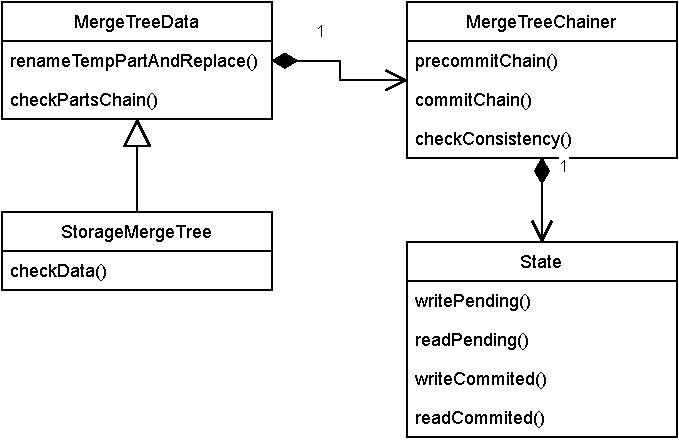
\includegraphics[scale=0.8]{img/classscheme.pdf}
	\caption{Диаграмма классов реализуемого метода.}
	\label{fig:classscheme}
\end{figure}

\subsection{Код объекта, отвечающего за построение цепи хеш-сумм}

Для проверки и расчета цепи хеш-сумм используется класс \\ \texttt{MergeTreeDataChainer}. Его интерфейс представлен в листинге \ref{code:interface}. Публичный интерфейс состоит из следующих методов:
\begin{enumerate}
    \item \texttt{precommitChain} --- проверяет, что текущая цепь хеш-сумм валидна и записывает в журнал значение новой. В качестве аргументов получает текущую цепь, элемент, который добавляется в цепь, вектор элементов, которые удаляются из цепи, а также блокировку на использование звеньев. Возвращает булево значение, было ли записано значение в журнал (не записывается в случае неверной цепочки на момент вызова метода).
    \item \texttt{checkConsistency} --- проверяет цепь. На вход получает набор звеньев, а также блокировку на использование звеньев.
    \item \texttt{commitChain} --- фиксирует значение цепи хеш-сумм, перенося его из журнала в файл цепи. На вход получает блокировку на использование звеньев.
\end{enumerate}

\pagebreak

\begin{lstlisting}[label=code:interface, caption={Класс \texttt{MergeTreeDataChainer}.}]
class MergeTreeDataChainer
{
    using Checksum = UInt64;

public:
    MergeTreeDataChainer(DiskPtr disk, String relative_storage_path, Poco::Logger * log = nullptr);
    bool precommitChain(DataParts & data_parts, const DataPartPtr & part_to_add,
        const DataPartsVector & parts_to_remove, const DataPartsLock & lock);
    CheckResult checkConsistency(const DataParts & data_parts, const DataPartsLock & /*lock*/);
    void setIgnoreOnInconsistency(const bool new_value) { ignore_on_inconsistency = new_value; }
    void setThrowOnInconsistency(const bool new_value) { throw_on_inconsistency = new_value; }
    void commitChain(const DataPartsLock & /*lock*/);

private:
    Checksum calculateChain(const DataParts & data_parts);
    static void transformToFutureState(DataParts & data_parts, const DataPartPtr & part_to_add,
        const DataPartsVector & parts_to_remove);
    void precommitChain(const DataParts & data_parts, const DataPartsLock & /*lock*/);
    void updateFromOnePart(SipHash & hash, const DataPart & data_parts);

    State state;
    Poco::Logger * log;
    bool throw_on_inconsistency = false;
    bool ignore_on_inconsistency = false;
};
\end{lstlisting}

Метод, отвечающий за проверки корректности цепи хеш-сумм, представлен в листинге \ref{code:validation}. Данный код сначала проверяет соответствие цепочки зафиксированному в файле значению. Если обнаруживается несовпадение, то результат сравнивается с значением из журнала. Если не совпадает со значением из журнала, то возвращается ошибка.

\pagebreak

\begin{lstlisting}[label=code:validation, caption={Валидация цепи хеш-сумм.}]
CheckResult MergeTreeData::MergeTreeDataChainer::checkConsistency(const DataParts & data_parts, const DataPartsLock & /*lock*/) {
    if (data_parts.size() == 0) {
        const auto pending = state.readPending(), commited = state.readCommited();
        return pending == 0 && commited == 0
            ? CheckResult("parts_chain", true, "")
            : CheckResult("parts_chain", false, "no parts, but not empty checksums: " + std::to_string(pending) + " and " + std::to_string(commited));
    }
    const auto checksum = calculateChain(data_parts);
    const auto commited = state.readCommited();
    if (commited == checksum)
        return CheckResult("parts chain", true, "");

    const auto pending = state.readPending();
    if (pending == checksum) {
        if (log)
            log->warning("parts chain is verified with pending value, rewriting commited");
        state.writeCommited(checksum);
        return CheckResult("parts chain", true, "");
    }
    return CheckResult("parts chain", false, "Parts chain is not valid!");
}
\end{lstlisting}

Сравнение цепей хеш-сумм сводится к сравнению 2 векторов. Код, рассчитывающий значение цепи хеш-сумм, представлен в листинге \ref{code:calcchain}. Цепь представляется вектором хешей, где хеш --- число размером 8 байт. Для расчета хешей используется хеш-функция \texttt{SipHash}. Для каждого очередного в качестве значения используются хеш-суммы всех файлов, имеющихся в звене, а также хеш-предыдущего звена (для первого звена используется 0).

\pagebreak

\begin{lstlisting}[label=code:calcchain, caption={Расчет цепи хеш-сумм.}]
MergeTreeData::MergeTreeDataChainer::Checksum
MergeTreeData::MergeTreeDataChainer::calculateChain(const DataParts & data_parts) {
    if (data_parts.size() == 0)
        return 0;
    Checksum prev = 0;
    for (const auto& part : data_parts) {
        SipHash hash{0, 0};
        hash.update(prev);
        updateFromOnePart(hash, *part);
        prev = hash.get64();
    }
    return prev;
}
void MergeTreeData::MergeTreeDataChainer::updateFromOnePart(SipHash & hash, const DataPart & data_part) {
    for (const auto& [file, checksum] : data_part.checksums.files) {
        hash.update(file);
        hash.update(checksum);
    }
}
\end{lstlisting}

Код метода \texttt{precommitChain} представлен в листинге \ref{code:precommitChain}. В данном методе происходят следующие действия:
\begin{enumerate}
    \item проверятся консистентность цепи для текущего списка активных звеньев;
    \item если проверка успешна, то к текущему списку добавляется звено на добавление, и удаляются звенья, которые требуется удалить;
    \item для нового состояние активных блоков высчитывается цепочка и записывается в журнал.
\end{enumerate}

\pagebreak

\begin{lstlisting}[label=code:precommitChain, caption={Метод \texttt{precommitChain}.}]
bool MergeTreeData::MergeTreeDataChainer::precommitChain(DataParts & data_parts,
    const DataPartPtr & part_to_add, const DataPartsVector & parts_to_remove, const DataPartsLock & lock) {
    if (!checkConsistency(data_parts, lock).success) {
        if (log)
            log->error("Parts chain is inconsistent (ignoring inconsistency: " + std::to_string(ignore_on_inconsistency) + ")");
        if (throw_on_inconsistency)
            throw Exception(ErrorCodes::LOGICAL_ERROR, "Parts chain is inconsistent and throw mode is set.");
        if (!ignore_on_inconsistency)
            return false;
    }
    transformToFutureState(data_parts, part_to_add, parts_to_remove);
    precommitChain(data_parts, lock);
    return true;
}
void MergeTreeData::MergeTreeDataChainer::precommitChain(const DataParts & data_parts, const DataPartsLock & /*lock*/) {
    state.writePending(calculateChain(data_parts));
}
void MergeTreeData::MergeTreeDataChainer::transformToFutureState(DataParts & data_parts,
    const DataPartPtr & part_to_add, const DataPartsVector & parts_to_remove) {
    data_parts.insert(part_to_add);
    for (const auto& part : parts_to_remove)
        data_parts.erase(part);
}
\end{lstlisting}

\subsection{Код изменения состояний активных блоков}

Как было описано в аналитической части и в схемах алгоритмов, улучшение метода хранения, которое позволяет доказывать неправомерное удаление, работает в тот момент, когда происходит изменения состояний блоков. Это происходит в функции \texttt{renameTempPartAndReplace} класса \texttt{MergeTreeData}. Код с использованием цепи хеш-сумм, описан в листингах \ref{code:updrename} и \ref{code:updrename2} в приложении А.

\subsection{Выводы}

В данном разделе были рассмотрены используемые инструменты и технологии, диаграмма классов для реализуемого метода, а также сама реализация.

\pagebreak